%==============================================================================
\chapter{In silico personalised rat heart contraction models: the role of $\Ca$ 
and sarcomere dynamics in diastolic heart failure}\label{cha:chapter4}
%==============================================================================
%
%
%
\section{Rat data}
We used healthy control and diseased rat data from experimental studies conducted by R{\o}e et al. \cite{Roe:2017}. Briefly, \textit{aortic banding} (\acs{AB}) was performed in male Wistar rats ($n=29$), while \textit{sham-operated} (\acs{SHAM}) rats ($n=23$) served as controls. \textit{In vivo} cardiac function was characterised by echocardiography six weeks after surgery. The criterion for inclusion in the AB group was posterior wall thickening ($>1.9$ mm). A cohort of rats ($n=8$, $n=15$ from SHAM, AB groups, respectively) underwent an examination with \textit{magnetic resonance imaging} (\acs{MRI}). Rats in the AB cohort showed a preserved systolic function (ejection fraction and fractional shortening). Concentric LV hypertrophy arose, as an increase in LV mass and wall thickness (WT) was observed. Moreover, evidence of reduced peak early diastolic velocity (e’) and increased early mitral inflow velocity / mitral annular early diastolic velocity (E/e’) confirmed an impaired diastolic function in the rats.

\vspace{0.2cm}
One representative cine MRI scan was obtained for both the SHAM and the AB rat cohorts. Each image set consisted of $47$ equally, $\SI{2.779}{\milli\second}$-spaced time frames. Example apicobasal slices are shown in Figure~\ref{fig:ratrepimag}, while MRI characteristics are reported in Table~\ref{tab:mrichar}.

\begin{figure}[hbt!]
    \myfloatalign
    \subfloat[SHAM]
    {\label{fig:ratrepimag-a}
    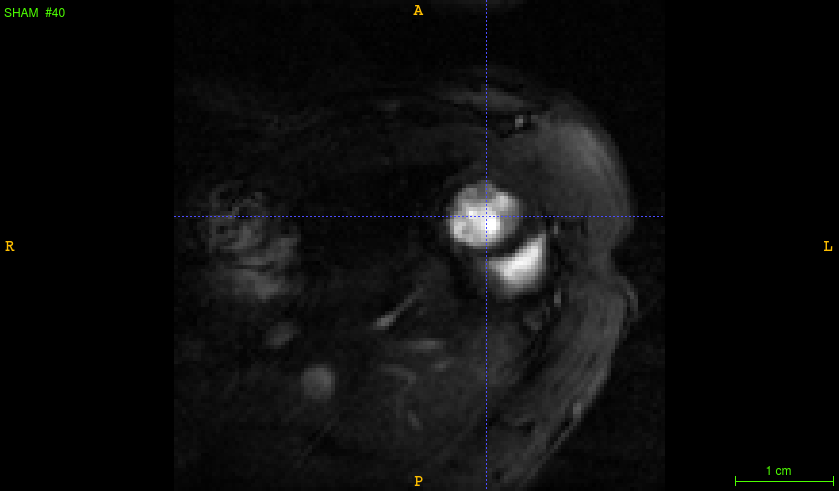
\includegraphics[width=.45\linewidth]{figures/chapter04/sham_image.png}}\quad
    \subfloat[AB]
    {\label{fig:ratrepimag-b}
    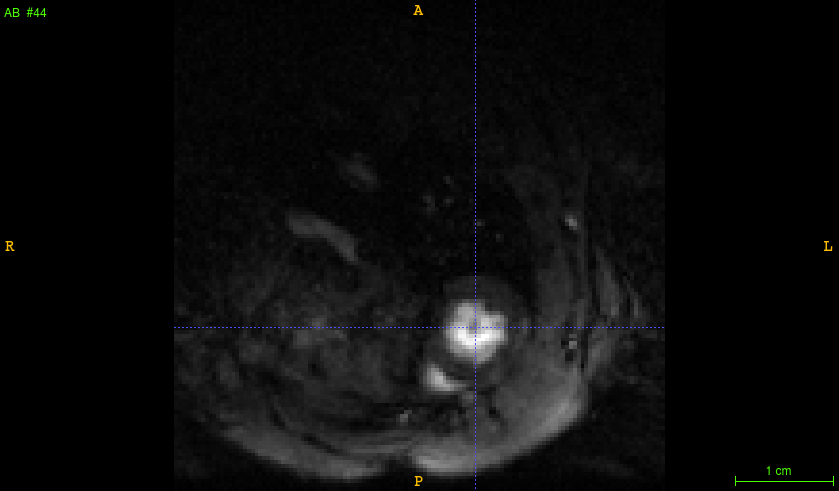
\includegraphics[width=.45\linewidth]{figures/chapter04/ab_image.png}}
    \caption{Rat representative MR Images.}\label{fig:ratrepimag}
\end{figure}

\begin{table}[hbt!]
    \myfloatalign
    \begin{tabularx}{\textwidth}{XXX}
    \toprule
    \tableheadline{Rat} & \multicolumn{2}{c}{\spacedlowsmallcaps{MRI characteristics}} \\
    \midrule   
    & \tableheadline{Size ($\#$voxels)} & \tableheadline{Voxel size ($\SI{}{\cubic\milli\meter}$)} \\
    \cmidrule{2-3}
    SHAM & $128\times 128\times 9$ & $0.39\times 0.39\times 1.5$ \\
    AB   & $128\times 128\times 9$ & $0.39\times 0.39\times 1.5$ \\
    \bottomrule
    \end{tabularx}
    \caption{MRI characteristics.}
    \label{tab:mrichar}
\end{table}

\vspace{0.2cm}
For each rat, we segmented the LV blood pool at each time frame and collected the corresponding volume estimates based on voxels size/count. This allowed to extract the entire experimental LV volume transient for each rat, displayed in Figure~\ref{fig:lvvexptransients}.

\begin{figure}[!h]
    \myfloatalign
    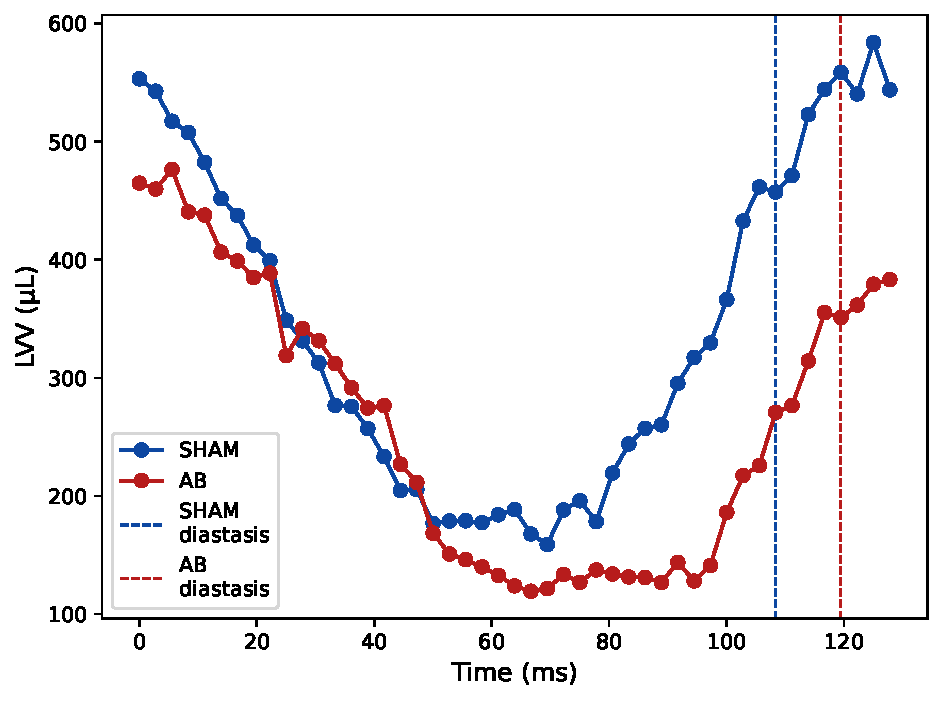
\includegraphics[width=0.8\textwidth]{figures/chapter04/lvv_experimental_transient.pdf}
    \caption{LV volume experimental transient obtained by segmenting the LV blood pool of $47$ consecutive time frames images for the SHAM (blue) and the AB (red) reference rat images. Dashed lines indicate approximately diastasis time during the cardiac cycle.}
    \label{fig:lvvexptransients}
\end{figure}

\vspace{0.2cm}
Time frames were numbered from $1$ to $47$. Frame $\#1$ was assumed to be moment when the heart enters the ejection phase of the cardiac cycle. In order to approximate the stress-free configuration for mechanics simulations, we selected a time frame halfway through diastole which could possibly represent cardiac diastasis (specifically frame $\#40$, $\#44$ for the SHAM, AB rats respectively). We segmented the entire biventricular anatomy at these time frames, comprising three main tags: the LV and RV blood pools and the surrounding myocardium. All the segmentations were performed manually using \texttt{ITK-SNAP} (v.$3.6.0$)~\cite{Yushkevich:2006}. Obtained segmentations are displayed in Figure~\ref{fig:ratrepseg} and estimated volumes are summarised in Table~\ref{tab:segmchar}.

\begin{figure}[bth]
    \myfloatalign
    \subfloat[SHAM]
    {\label{fig:ratrepseg-a}
    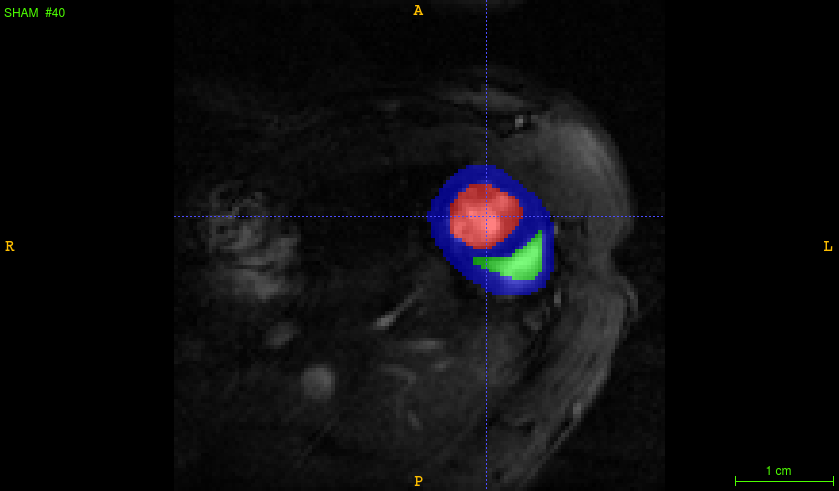
\includegraphics[width=.45\linewidth]{figures/chapter04/sham_segmentation.png}}\quad
    \subfloat[AB]
    {\label{fig:ratrepseg-b}
    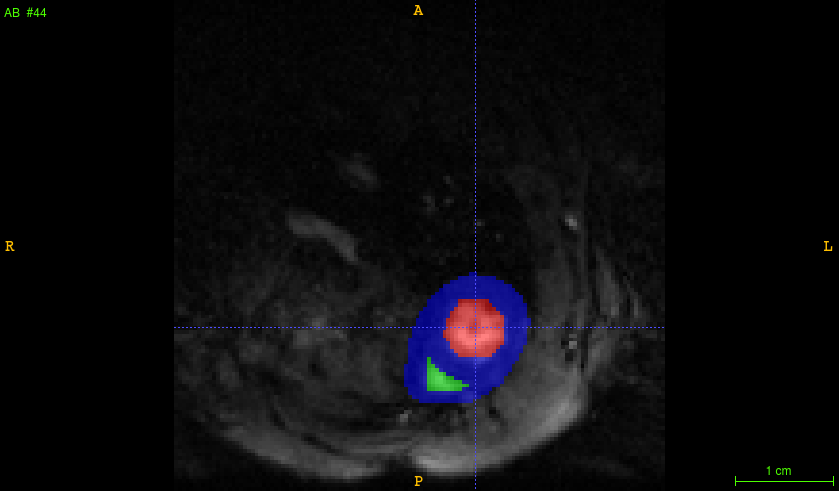
\includegraphics[width=.45\linewidth]{figures/chapter04/ab_segmentation.png}}
    \caption{Rat representative MRI scans segmentations. LV and RV blood pools and myocardium are tagged with respectively red, green and blue colours.}\label{fig:ratrepseg}
\end{figure}

\begin{table}[hbt!]
    \myfloatalign
    \begin{tabularx}{\textwidth}{XXXX}
    \toprule
    \tableheadline{Rat} & \multicolumn{3}{c}{\spacedlowsmallcaps{Segmentation characteristics}} \\
    \midrule   
    & \tableheadline{LV ($\SI{}{\cubic\milli\meter}$)} & \tableheadline{RV ($\SI{}{\cubic\milli\meter}$)} & \tableheadline{Myocardium ($\SI{}{\cubic\milli\meter}$)} \\
    \cmidrule{2-4}
    SHAM & $459.14$ & $417.94$ & $1127.93$ \\
    AB   & $357.97$ & $212.17$ & $1181.72$ \\
    \bottomrule
    \end{tabularx}
    \caption{Segmentation tags volume estimates based on voxels size/count.}
    \label{tab:segmchar}
\end{table}


%
%
%
$8$ LHDs of $1,024$ input parameter points each were simulated and the successfully completed simulations were collected to form the training dataset, with final size of $825$ and $850$ points for the SHAM and AB models, respectively. The low number of successful runs relates to a combination of failure of the mechanics simulations converging or completing a full cardiac cycle, which may happen if the contraction is insufficient to reach the aortic pressure. One GPE was trained for each output feature, for a total of $12$ GPEs. The obtained cross-validation $R^2$ test scores (GPEs' accuracy) are reported in Table~$1$ in the Supplementary materials. Emulator evaluation at a new parameter set took $\sim 1.2$ seconds against a full simulator single-core run of $\sim 4$ hours, for a total gained speedup of $12,000$ fold.

\begin{table}[!ht]
    \myfloatalign
    \begin{tabularx}{\textwidth}{XXX}
    \toprule
    \tableheadline{LV feature} & \tableheadline{$R^2$} & \tableheadline{$ISE_2 (\SI{}{\percent})$} \\
    \midrule
    $\textrm{EDV}$    & $0.9712 \pm 0.0046$ & $87.7576 \pm 1.1752$ \\
    $\textrm{ESV}$    & $0.9736 \pm 0.0023$ & $86.4242 \pm 2.5310$ \\
    $\textrm{EF}$     & $0.9342 \pm 0.0155$ & $87.6364 \pm 2.4424$ \\
    $\textrm{IVCT}$   & $0.9658 \pm 0.0122$ & $88.0000 \pm 4.5094$ \\
    $\textrm{ET}$     & $0.9408 \pm 0.0054$ & $88.2424 \pm 1.6531$ \\
    $\textrm{IVRT}$   & $0.9135 \pm 0.0128$ & $87.6364 \pm 4.3804$ \\
    $\textrm{Tdiast}$ & $0.9412 \pm 0.0056$ & $86.6667 \pm 1.9917$ \\
    $\textrm{PeakP}$  & $0.9867 \pm 0.0027$ & $86.7879 \pm 1.0427$ \\
    $\textrm{Tpeak}$  & $0.9659 \pm 0.0117$ & $85.6970 \pm 5.8207$ \\
    $\textrm{ESP}$    & $0.9973 \pm 0.0004$ & $86.6667 \pm 2.2350$ \\
    $\textrm{maxdP}$  & $0.9792 \pm 0.0064$ & $86.6667 \pm 4.8937$ \\
    $\textrm{mindP}$  & $0.7437 \pm 0.0283$ & $93.4545 \pm 1.6442$ \\
    \bottomrule
    \end{tabularx}
    \caption{The SHAM rat GPEs' accuracy. The GPEs' accuracy was evaluated using the average $R^{2}$ score and $ISE_2$ obtained with a $5$-fold cross-validation.}
    \label{tab:gpescores1_sham}
\end{table}

\begin{figure}[!ht]
    \myfloatalign
    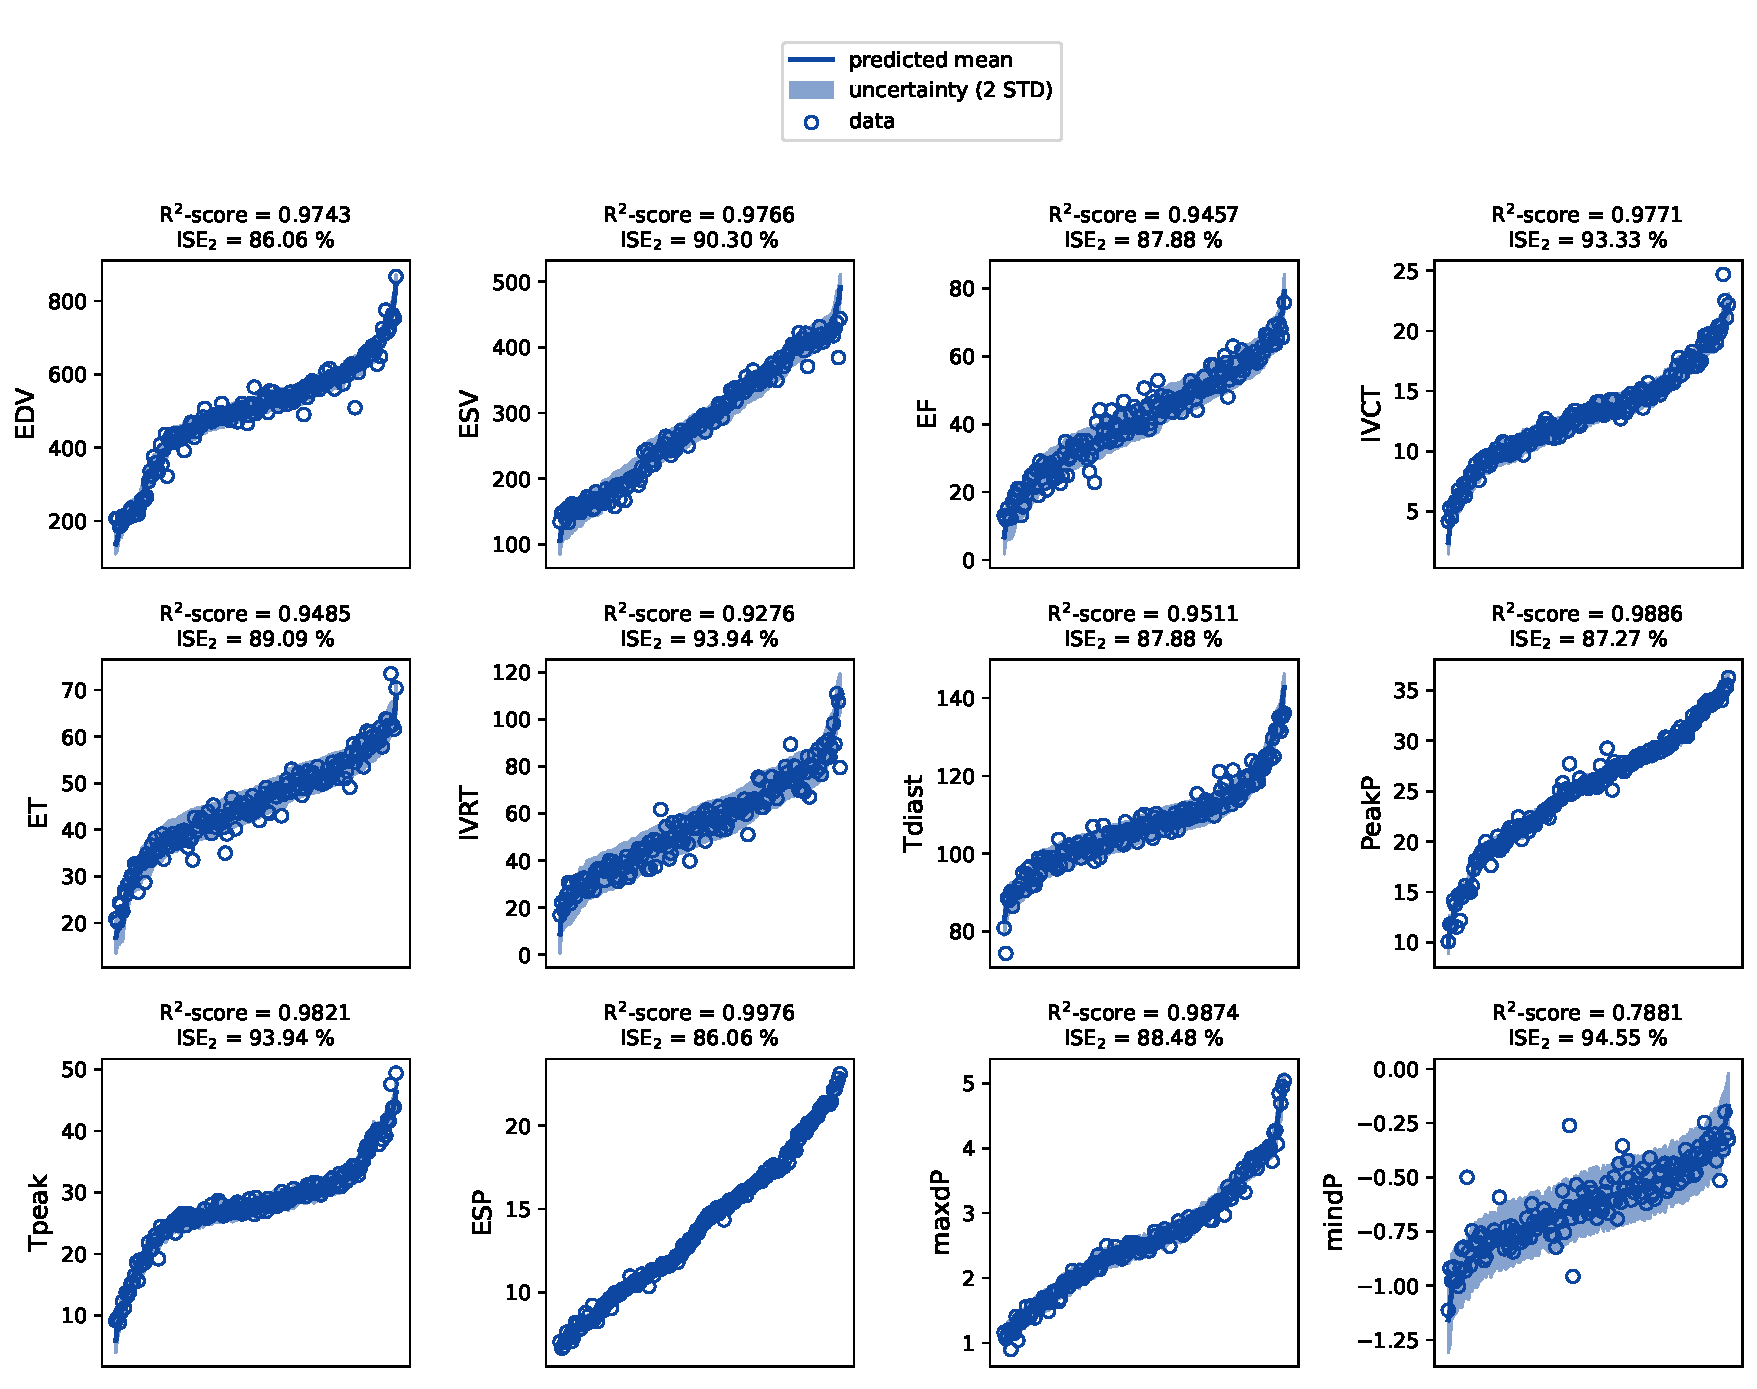
\includegraphics[width=\textwidth]{figures/chapter04/bgpes_vs_bsplit_sham.pdf}
    \caption{For each LV feature, the GPE with the highest $R^2$ split test score is used to make predictions at the respective left-out subset of test points. Predictions are sorted in ascending order for the sake of a better visualisation and joined with a thick blue line, and the respective observations (empty dots) are sorted accordingly. $2$ STD confidence intervals (shaded regions) are also plotted around predicted mean lines.}
    \label{fig:gpesexampleinferencesham}
\end{figure}

\begin{table}[!ht]
    \myfloatalign
    \begin{tabularx}{\textwidth}{XXX}
    \toprule
    \tableheadline{LV feature} & \tableheadline{$R^2$} & \tableheadline{$ISE_2 (\SI{}{\percent})$} \\
    \midrule
    $\textrm{EDV}$    & $0.9461 \pm 0.0273$ & $87.8824 \pm 4.0516$ \\
    $\textrm{ESV}$    & $0.9714 \pm 0.0050$ & $87.2941 \pm 2.3705$ \\
    $\textrm{EF}$     & $0.9661 \pm 0.0101$ & $86.2353 \pm 3.6376$ \\
    $\textrm{IVCT}$   & $0.9906 \pm 0.0021$ & $84.4706 \pm 2.5123$ \\     
    $\textrm{ET}$     & $0.9593 \pm 0.0159$ & $89.2941 \pm 3.4979$ \\
    $\textrm{IVRT}$   & $0.8559 \pm 0.0165$ & $85.8824 \pm 1.7842$ \\
    $\textrm{Tdiast}$ & $0.9473 \pm 0.0197$ & $88.1176 \pm 4.0652$ \\
    $\textrm{PeakP}$  & $0.9871 \pm 0.0077$ & $85.2941 \pm 2.1372$ \\
    $\textrm{Tpeak}$  & $0.9542 \pm 0.0150$ & $86.0000 \pm 7.7092$ \\
    $\textrm{ESP}$    & $0.9959 \pm 0.0024$ & $86.2353 \pm 2.5936$ \\
    $\textrm{maxdP}$  & $0.9860 \pm 0.0039$ & $87.4118 \pm 3.0814$ \\
    $\textrm{mindP}$  & $0.7474 \pm 0.0687$ & $89.7647 \pm 2.3705$ \\
    \bottomrule
    \end{tabularx}
    \caption{The AB rat GPEs' accuracy. The GPEs' accuracy was evaluated using the average $R^{2}$ score and $ISE_2$ obtained with a $5$-fold cross-validation.}
    \label{tab:gpescores1_ab}
\end{table}

\begin{figure}[!ht]
    \myfloatalign
    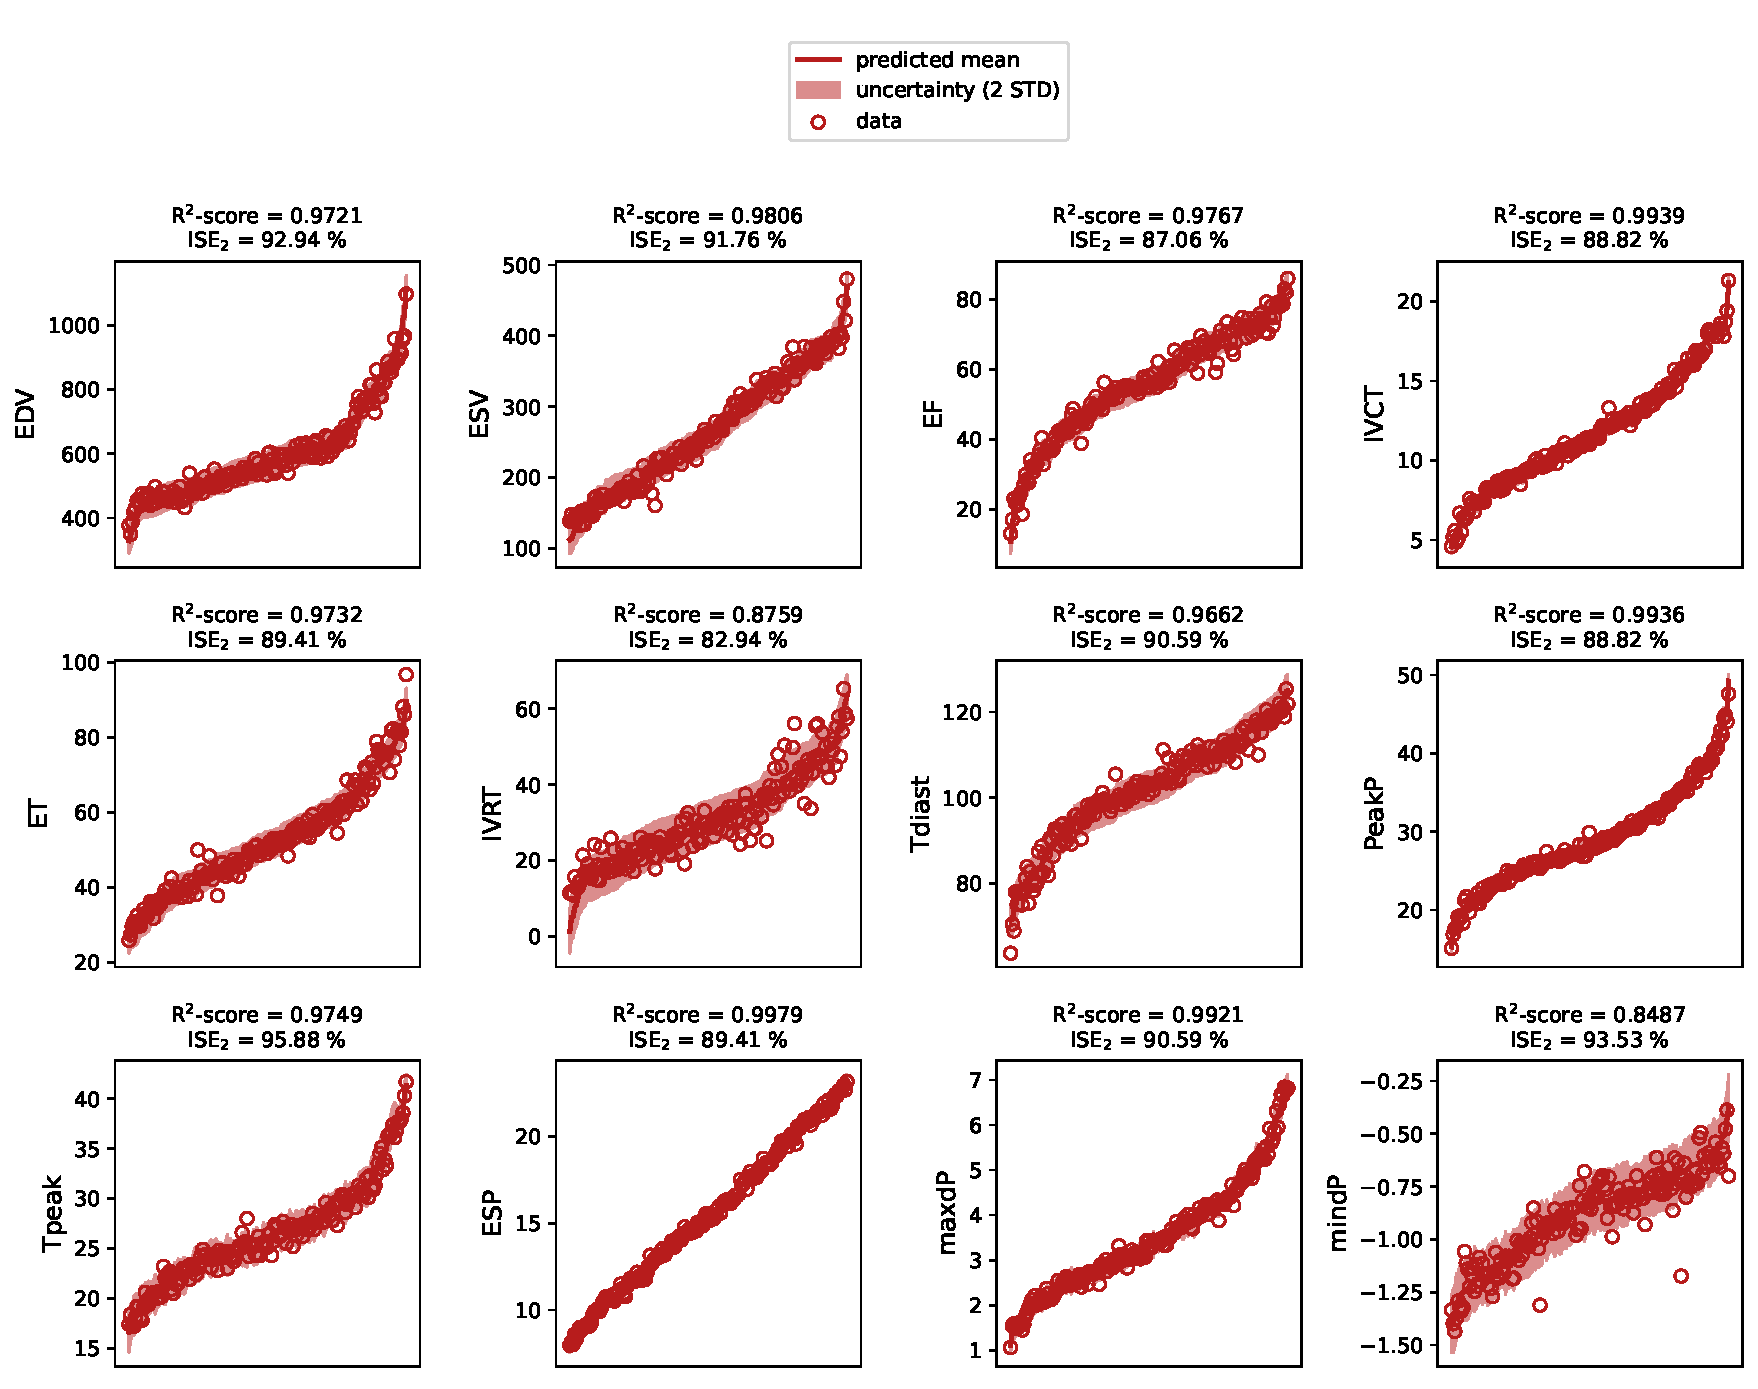
\includegraphics[width=\textwidth]{figures/chapter04/bgpes_vs_bsplit_ab.pdf}
    \caption{For each LV feature, the GPE with the highest $R^2$ split test score is used to make predictions at the respective left-out subset of test points. Predictions are sorted in ascending order for the sake of a better visualisation and joined with a thick blue line, and the respective observations (empty dots) are sorted accordingly. $2$ STD confidence intervals (shaded regions) are also plotted around predicted mean lines.}
    \label{fig:fig:gpesexampleinferencesham}
\end{figure}

\vspace{0.2cm}
For this study, the target organ-scale features' mean and standard deviation values for HM come from two different sources. Whenever it was not possible to get information about a specific organ-scale feature from the available MRI data \cite{Roe2017}, the information was obtained from available literature data from experimental studies performed in male rats at body temperature with abdominal/ascending aortic banding \cite{Nemeth2016, Sato1990, Schunkert1995, Loot2005, Liu2014, Ku2014, Ruppert2018, Schunkert1990, Ruppert2016}. In particular, EDV, ESV, ET and IVRT features were immediately available from the MRI data, while information about PeakP, maxdP and mindP features was collected from literature. Mean and standard deviation values for the volume-related features come from recordings performed on the cohort of rats ($n=8$, $n=15$ from SHAM, AB groups, respectively) that underwent MRI examination \cite{Roe2017}. Mean and standard deviation values for each pressure-related feature were calculated from the set of experimental mean values collected from each of above-mentioned literature studies. We did not have specific values for IVCT, Tdiast, Tpeak and ESP, and we chose not to match EF explicitly as this is derived form EDV and ESV. This resulted in $7$ organ-scale phenotypes (see Table \ref{tab:values2match}) used to constrain the model parameters.

\begin{table}[!ht]
    \myfloatalign
    \begin{tabularx}{\textwidth}{lrrl}
    \toprule
    \tableheadline{LV feature} & \multicolumn{2}{c}{\spacedlowsmallcaps{Exp. variability}} & \tableheadline{Reference} \\
    \midrule
                                                      & \tableheadline{SHAM} & \tableheadline{AB}                 & \\
    \midrule
    $\textrm{EDV}^{*}$                  & $508.80 \pm 39.01$ & $466.50 \pm 37.10$ & \cite{Roe:2017} \\
    $\textrm{ESV}^{*}$                  & $154.60 \pm 16.53$ & $125.60 \pm 23.40$ & \cite{Roe:2017} \\
    $\textrm{ET}^{*}$                 & $51.21  \pm  1.85$ & $54.72  \pm  1.85$ & \cite{Roe:2017} \\
    $\textrm{IVRT}^{*}$                 & $20.55  \pm  1.85$ & $41.11  \pm  1.85$ & \cite{Roe:2017} \\
    $\textrm{PeakP}^{**}$                  & $16.66  \pm  1.02$ & $21.66  \pm  0.69$ & \cite{Sato:1990, Schunkert:1990, Schunkert:1995, Loot:2005, Ku:2014, Liu:2014, Nemeth:2016, Ruppert:2016, Ruppert:2018} \\
    $\textrm{maxdP}^{**}$ & $1.14   \pm  0.25$ & $1.24   \pm  0.24$ & \cite{Sato:1990, Schunkert:1990, Schunkert:1995, Loot:2005, Ku:2014, Liu:2014, Nemeth:2016, Ruppert:2016, Ruppert:2018} \\
    $\textrm{mindP}^{**}$ & $-1.00  \pm  0.23$ & $-1.16  \pm  0.23$ & \cite{Sato:1990, Schunkert:1990, Schunkert:1995, Loot:2005, Ku:2014, Liu:2014, Nemeth:2016, Ruppert:2016, Ruppert:2018} \\
    \bottomrule
    \end{tabularx}
    \caption{Left ventricular features' target mean and standard deviation values. One asterisk $(\,\,)^*$ features values come directly from the available MRI data. Two asterisks $(\,\,)^{**}$ features values come from literature experimental studies.}
    \label{tab:values2match}
\end{table}

\newpage
\begin{landscape}
\begin{table}
    \vspace{-\marginparsep}
    \vspace{-\marginparwidth}
    \begin{tabularx}{2\textwidth}{llllll}
    \toprule
    \tableheadline{Parameter} & \tableheadline{Units} & \multicolumn{2}{l}{\spacedlowsmallcaps{Value from experimental papers}} & \multicolumn{2}{l}{\spacedlowsmallcaps{Value from modelling papers}} \\ \midrule
     & & \tableheadline{Range} & \tableheadline{Reference} & \tableheadline{Range} & \tableheadline{Reference} \\ \midrule
    $\Caif$ & $\SI{}{\micro\Molar}$                 & $-$ & $-$ & $[0.8,\,1.56]$ & \cite{Land:2012*a, Lewalle:2018, Niederer:2006, Wei-Dong-Gao:1994, Gao:1995, Backx:1995} \\
    $\koff$                                & $\SI{}{\per\milli\second}$            & $[0.0013,\,1.2]$ & \cite{Rosenfeld:1985, Tikunova:2004, Davis:2007} & $[0.05,\,0.2]$ & \cite{Land:2012*a, Lewalle:2018, Niederer:2006} \\
    $\kxb$                                  & $\SI{}{\per\milli\second}$            & $0.1$ & \cite{Blanchard:1999, Stull:2002} & $[0.008,\,0.2]$ & \cite{Land:2012*a, Lewalle:2018} \\
    $\tref$                                 & $\SI{}{\kilo\pascal}$                 & $-$ & $-$ & $[20,\, 160]$ & \cite{Land:2012*a, Lewalle:2018, Niederer:2006, Niederer:2009, Blanchard:1999, Stuyvers:2002, Palmer:2004, Kreutziger:2011, Rice:2008, Bovendeerd:2009} \\
    $\p$                                                & $\SI{}{\kilo\pascal}$                 & $[0.2,\,1.4]$ & \cite{Nemeth:2016, Sato:1990, Schunkert:1995, Loot:2005, Liu:2014, Ku:2014, Ruppert:2018, Schunkert:1990, Ruppert:2016} & $1.0$ & \cite{Land:2012*a, Lewalle:2018} \\
    $\pao$                                              & $\SI{}{\kilo\pascal}$                 & $[12,\,21]$ & \cite{Nemeth:2016, Ku:2014, Ruppert:2018, Kovacs:2015, Lee:2017, Olah:2015, Ruppert:2016, Toledo:2017} & $[8,\,9]$ & \cite{Land:2012*a, Lewalle:2018} \\
    $\Z$                                                & $\SI{}{\mmHg\second\per\milli\litre}$ & $[1.5,\,16]$ & \cite{Kobayashi:1996, Levy:1988, Zuckerman:1989, Lin:2004, Yin:1980, Ioannou:2009, Chang:2015} & $[6,\,20]$ & \cite{Land:2012*a, Lewalle:2018, Westerhof:1991} \\
    $\Cone$                                              & $\SI{}{\kilo\pascal}$                 & $[0.1,\,3.0]$ & \cite{Nordbo:2014} (review paper) & $[0.4,\,1.1]$ & \cite{Land:2012*a, Lewalle:2018, Niederer:2009, Omens:1993} \\
    \bottomrule
    \end{tabularx}
    \caption{SHAM rat model input parameters' ranges. The initial range of each parameter will be given by the union of experimental and modelling papers' ranges, intersected with the range resulting for the AB rat model (Table~\ref{tab:abranges}).}
    \label{tab:shamranges}
\end{table}
\end{landscape}

\newpage
\begin{landscape}
\begin{table}
    \vspace{-\marginparsep}
    \vspace{-\marginparwidth}
    \begin{tabularx}{2\textwidth}{llllll}
    \toprule
    \tableheadline{Parameter} & \tableheadline{Units} & \multicolumn{2}{l}{\spacedlowsmallcaps{Value from experimental papers}} & \multicolumn{2}{l}{\spacedlowsmallcaps{Value from modelling papers}} \\ \midrule
     & & \tableheadline{Range} & \tableheadline{Reference} & \tableheadline{Range} & \tableheadline{Reference} \\ \midrule
    $\Caif$ & $\SI{}{\micro\Molar}$                 & $-$ & $-$ & $[0.8,\,1.0]$ & \cite{Lewalle:2018} \\
    $\koff$                                & $\SI{}{\per\milli\second}$            & $-$ & $-$ & $0.1$ & \cite{Lewalle:2018} \\
    $\kxb$                                  & $\SI{}{\per\milli\second}$            & $-$ & $-$ & $0.02$ & \cite{Lewalle:2018} \\
    $\tref$                                 & $\SI{}{\kilo\pascal}$                 & $-$ & $-$ & $120$ & \cite{Lewalle:2018} \\
    $\p$                                                & $\SI{}{\kilo\pascal}$                 & $[0.3,\,1.6]$ & \cite{Nemeth:2016, Sato:1990, Schunkert:1995, Loot:2005, Liu:2014, Ku:2014, Ruppert:2018, Schunkert:1990, Ruppert:2016} & $1.0$ & \cite{Lewalle:2018} \\
    $\pao$                                              & $\SI{}{\kilo\pascal}$                 & $[21,\,26]$ & \cite{Nemeth:2016, Ku:2014, Ruppert:2018, Ruppert:2016} & $[7,\,20]$ & \cite{Lewalle:2018} \\
    $\Z$                                                & $\SI{}{\mmHg\second\per\milli\litre}$ & $[5.5,\,23]$ & \cite{Kobayashi:1996, Yin:1980, Ioannou:2009} & $9.5$ & \cite{Lewalle:2018} \\
    $\Cone$                                              & $\SI{}{\kilo\pascal}$                 & $-$ & $-$ & $[0.2,\,1.6]$ & \cite{Lewalle:2018} \\
    \bottomrule
    \end{tabularx}
    \caption{AB rat model input parameters' ranges. The initial range for each parameter will be given by the union of experimental and modelling papers' ranges, intersected with the range resulting for the SHAM rat model (Table \ref{tab:shamranges}).}
    \label{tab:abranges}
\end{table}
\end{landscape}
